% Manual template (AAT2), see docs/HowToDoc.md
% Build (in docs/manual):  pdflatex ManualMomentNoise.tex   (twice, for the references)
% The PDF is copied into the release zips by the GitHub workflow.
\documentclass[12pt]{article}
\usepackage[utf8]{inputenc}
\usepackage[T1]{fontenc}
\usepackage[top=2cm, bottom=2cm, left=2cm, right=2cm]{geometry}
\usepackage{graphicx}
\usepackage{xcolor}
\usepackage{amsmath}
\usepackage{hyperref}
\hypersetup{colorlinks=true, linkcolor=red, urlcolor=red, pdftitle={MomentNoise Documentation}}

% ---- change these ------------------------------------------------------------
\newcommand{\pluginversion}{0.1.0}   % the version in CMakeLists.txt
\newcommand{\pluginauthor}{Joerg Bitzer}
\newcommand{\sourceurl}{https://github.com/JoergBitzer/noise_moments}
% -------------------------------------------------------------------------------

\title{MomentNoise Documentation}
\author{License: CC-BY 4.0}
\date{\today, for MomentNoise \pluginversion}

\begin{document}
\maketitle

\section{Introduction}
MomentNoise is a noise generator whose amplitude distribution can be changed: besides the level,
you set the \emph{skewness} (asymmetry) and the \emph{excess kurtosis} (tail weight) of the noise. The
default is Gaussian (normal) noise at $-24$\,dBFS RMS. The lower half of the window shows the
theoretical probability density function (pdf) of the noise. Together with its companion plug-in
AmplitudeHistogram, which measures the histogram of a signal, it shows how the statistics of a
signal and its histogram belong together.

\textbf{Warning:} heavy-tailed noise (large excess kurtosis) has rare peaks far above its RMS level.
At $-24$\,dBFS RMS, skewness 2 and excess kurtosis 15, single peaks reach about $+5$\,dBFS. Lower the
level before you listen to such settings.

MomentNoise is a generator: the input signal is replaced by the noise (independent noise in every
channel).

\section{Installation}
The downloaded file is a zip file. It contains the plug-in (.vst3; on macOS also the AU,
.component), the Standalone application, a ReadMeFirst.txt, the licence files and this manual.
Copy the plug-in to the right place and let your DAW rescan its plug-ins.

\begin{verbatim}
Windows (VST3):  C:\Program Files\Common Files\VST3
Mac (VST3):      /Users/yourUSERNAME/Library/Audio/Plug-Ins/VST3
Mac (AU):        /Users/yourUSERNAME/Library/Audio/Plug-Ins/Components
Linux (VST3):    /home/yourUSERNAME/.vst3
\end{verbatim}

The macOS version is not signed with an Apple Developer ID. If macOS reports that the plug-in
is damaged or cannot be opened, remove the quarantine flag in the Terminal, e.g.
\texttt{xattr -cr \textasciitilde/Library/Audio/Plug-Ins/VST3/MomentNoise.vst3}.

\subsection{Presets and settings}
The presets (plain XML files) and the settings file (\texttt{user.settings}: day/night theme)
are stored in this folder -- delete it to remove MomentNoise completely:
\begin{verbatim}
Windows: C:\Users\yourUSERNAME\AppData\Roaming\Jade\_Hochschule\MomentNoise
Mac:     /Users/yourUSERNAME/Library/Audio/Presets/Jade\_Hochschule/MomentNoise
Linux:   /home/yourUSERNAME/.config/Jade\_Hochschule/MomentNoise
\end{verbatim}

\section{How to use}
\begin{center}
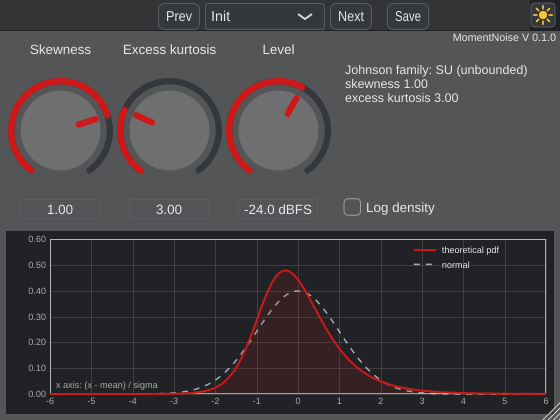
\includegraphics[width=0.8\textwidth]{images/GUI.png}
\end{center}
\begin{enumerate}
    \item \textbf{Preset handler}: Prev/Next step through the presets. To save a new preset,
    type a name and press Save. Save turns red when you change a parameter of the displayed
    preset; press it to update the preset. To delete a preset, delete its XML file.
    \item \textbf{Day/night}: switches between the night (dark) and the day (light) theme.
    \item \textbf{Skewness} ($-2 \dots 2$): the 3rd standardized moment. 0 is symmetric; positive values
    give a long tail towards positive amplitudes, negative values towards negative amplitudes.
    \item \textbf{Excess kurtosis} ($-1.5 \dots 15$): the 4th standardized moment minus 3. 0 is Gaussian;
    negative values give light tails (uniform noise: $-1.2$), positive values heavy tails with rare
    large peaks (Laplace: 3). Every distribution has an excess kurtosis above
    $\text{skewness}^2 - 2$; MomentNoise keeps a distance of 0.5 to this bound and raises smaller values
    (the info text says so).
    \item \textbf{Level}: RMS level (standard deviation) of the noise in dBFS.
    \item \textbf{Info text}: the Johnson family used (see section~\ref{sec:how}) and the skewness and
    excess kurtosis that were reached.
    \item \textbf{Log density}: the density axis of the display logarithmic (5 decades) or linear. The
    tails, where the kurtosis shows, are only visible in the logarithmic view.
    \item \textbf{Display}: the theoretical pdf (red) over the standardized amplitude
    $(x - \text{mean})/\sigma$ from $-6\sigma$ to $6\sigma$, the normal pdf as dashed reference.
    AmplitudeHistogram uses the same axes, so both displays can be compared directly.
\end{enumerate}

\section{Controls}\label{sec:controls}
All controls, their range and default value. Rest the mouse on a control to see its
description as a tooltip.

\begin{center}
\small
% generated from the code: MomentNoise_Tester --manual tex > controls.tex (see docs/HowToDoc.md)
\begin{tabular}{p{0.2\textwidth}p{0.22\textwidth}p{0.12\textwidth}p{0.36\textwidth}}
\hline
Control & Range & Default & Description \\
\hline
Skewness & -2.00 - 2.00 & 0.00 & Asymmetry of the amplitude distribution (3rd standardized moment): 0 = symmetric, positive = long tail towards positive amplitudes. \\
Excess kurtosis & -1.50 - 100.00 & 0.00 & Tail weight (4th standardized moment minus 3): 0 = Gaussian, negative = light tails (uniform: -1.2), positive = heavy tails, rare large peaks (Laplace: 3). At least skewness squared - 1.5, smaller values are raised. \\
Level & -60.0 dBFS - 0.0 dBFS & -24.0 dBFS & RMS level of the noise (its standard deviation). Heavy tails give peaks far above the RMS level: they may exceed 0 dBFS. \\
Log density & Off - On & Off & Density axis of the display logarithmic (shows the tails) or linear. \\
\hline
\end{tabular}

\end{center}

\section{How it works}
\label{sec:how}
The noise comes from the \emph{Johnson system} of distributions (N.\,L.~Johnson, 1949). A standard
normal random variable $z$ is transformed into
\[ x = \xi + \lambda \, y(z) \]
with one of four families:
\begin{center}
\begin{tabular}{lll}
SN (normal) & $y = z$ & skewness 0, excess kurtosis 0\\
SL (lognormal) & $y = e^{z/\delta}$ & on the ``lognormal line''\\
SU (unbounded) & $y = \sinh(z/\delta) + t\cosh(z/\delta)$ & above the lognormal line (heavy tails)\\
SB (bounded) & $y = 1/(e^{-z/\delta} + c)$ & below the lognormal line (light tails, bounded)\\
\end{tabular}
\end{center}
($t = \tanh(\gamma/\delta)$ and $c = e^{-\gamma/\delta}$ are Johnson's parameter $\gamma$ in a form that
cannot overflow.) Together the families cover every possible pair of skewness and excess kurtosis, so
both can be set independently. When a parameter changes, a background thread searches $\delta$ and
$t$ (or $c$) so that the moments of $y$, computed by numerical integration over $z$, have the wanted
skewness and excess kurtosis (two nested root searches, at most about 80\,ms). $\xi$ and $\lambda$ then
give mean 0 and variance 1; a negative skewness mirrors the distribution. The pdf of the display
follows from the change of variables, $p(x) = \varphi(z)\,|dz/dx|$.

For every sample a Gaussian random number $z$ is drawn and transformed; the level scales the result
(smoothed over 20\,ms).

\section{Source code}
MomentNoise is open source. You find the source code here:\newline
\url{\sourceurl}. Please report bugs there, too.

\section{Legal stuff}
For this documentation the CC-BY 4.0 licence is valid. Copyright holder is \pluginauthor.
The source code of the plug-in is under the MIT licence. The plug-in binaries contain JUCE
(used under the AGPLv3), the VST3 SDK (MIT) and, on macOS, the Audio Unit SDK (Apache 2.0);
the binaries as a whole are distributed under the AGPLv3.

\begin{itemize}
    \item Microsoft\textsuperscript{\textregistered}, Windows\textsuperscript{\textregistered}
    are trademarks of the Microsoft group of companies.
    \item Mac\textsuperscript{\textregistered} is a trademark of Apple Inc.
    \item VST\textsuperscript{\textregistered} is a registered trademark of Steinberg Media
    Technologies GmbH.
\end{itemize}

\end{document}
